

\chapter{Metodologia}
\label{metodologia}




\section{Caracterização da Pesquisa}

O percurso metodológico caracteriza-se como uma pesquisa aplicada, com abordagem mista (quantitativa e qualitativa), de natureza exploratória e com análise predominantemente indutiva, aplicando métodos de análise documental envolvendo os planos de aula e ensino para verificar no planejamento docente a previsão de adoção de alguma ferramenta tecnológica educacional e ou a transdisciplinaridade. A baixo na Figura \ref{fig:classificacao_metodologica} um esquema da classificação metodológica da pesquisa:

\begin{figure}[h!]
    \caption{Classificação metodológica}
    \centering
    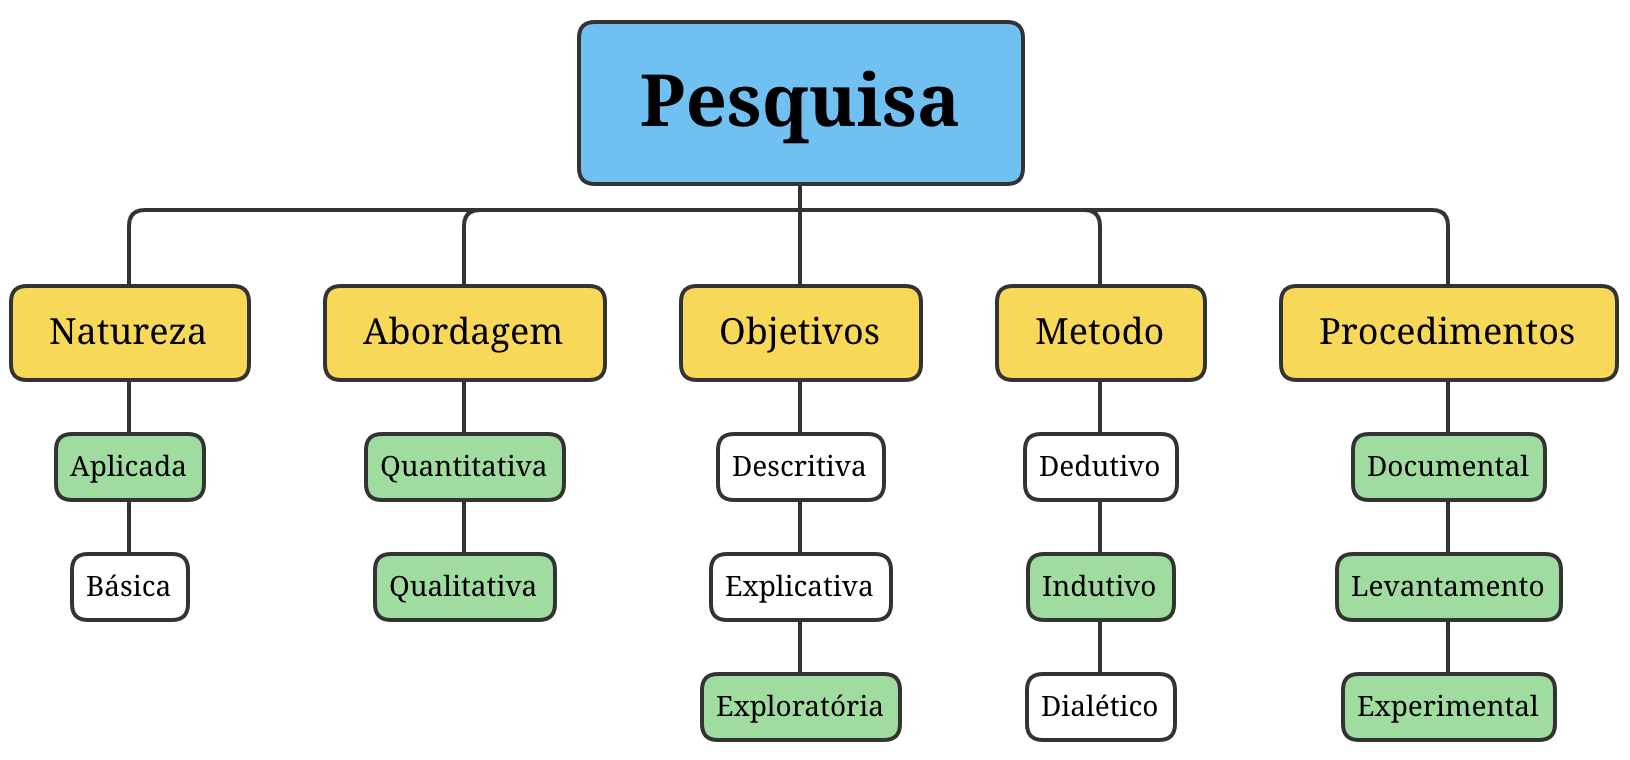
\includegraphics[scale=0.5]{figuras/metodologia.png}
    \label{fig:classificacao_metodologica}
    \legend{Fonte: Adaptado de \citeonline{marconi2017fundamentos}}
\end{figure}







\section{Local da Pesquisa}
\label{local_pesquisado}

O estudo foi conduzido no Instituto Federal do Amapá (IFAP), Campus Macapá, único campus da instituição que oferece o curso de Licenciatura em Matemática. O curso teve seu ato de criação pela Resolução nº 17/2016/CONSUP/IFAP, de 09 de maio de 2016 – Aprova o Ato de Criação, Autorização e Funcionamento do Curso Superior de Licenciatura em Matemática, modalidade presencial do Campus Macapá \cite{ifap2022}.

Também em 2016 publicou-se a Resolução nº 49/2016/CONSUP/IFAP, de 18 de outubro de 2016 – Aprova o Projeto Pedagógico do Curso Superior de Licenciatura em Matemática, modalidade presencial do Campus Macapá \cite{ifap2022}.









\section{Sujeitos da Pesquisa}
\label{sujeitos_pesquisa}

A população pesquisada será os docentes do curso, porém a amostragem corresponde apenas aos docentes que ministram os componentes não pedagógicos (componentes das áreas técnicas) totalizando 13 docentes, ressaltar que para acesso aos planos de aula e ensino deve-se adentrar ao Setor Pedagógico para obter acesso aos documentos e a busca fica restrita ao intervalo entre os anos de 2016 até 2021.


As informações serão coletadas por uma plataforma única para a coleta de dados ou utilizando um procedimento de amostragem em cadeia, como a metodologia conhecida como “bola de neve” (\textit{snowball sampling}) adaptada à plataformas virtuais \cite{szwarcwald2021convid}. O método “bola de neve” é um procedimento de amostragem não probabilístico, que funciona a partir da indicação de um grupo inicial de pessoas que fazem parte da população-alvo (denominadas de sementes), que indicam pares do mesmo grupo populacional, e assim sucessivamente, semelhante à formação de uma bola de neve \cite{szwarcwald2021convid}.





\subsection{Descrição dos Sujeitos}
\label{descricao_sujeitos}


Os docentes, sujeitos da pesquisa são caracterizados pelo eixo de disciplinas ligados ao curso de licenciatura em matemática de ambos os sexos e tempo de experiência diversos até mesmo em outras de áreas do conhecimento. Ressaltar que apenas os docentes do Campus Macapá que ministram componentes específicos da matemática inicialmente participaram indicando outros seguindo docentes seguindo o método da bola de neve.








\subsection{Critérios de Inclusão e Exclusão}
\label{criterios_sujeitos}

Como critérios de inclusão para todos os participantes  é dar o aceite concordando com o Termo de Esclarecimento Livre Esclarecido (TCLE):
\begin{itemize}
    \item Ser docente efetivo, substituto ou temporário do IFAP ou em instituição com o curso de Licenciatura em Matemática;
    \item Ministrar componentes no curso de Licenciatura em Matemática;
    \item Componente ministrado seja da área técnica ou superior;
    \item Atuado no período entre 2016 até 2021.
\end{itemize}




\section{Aspectos Éticos}
\label{aspectos_eticos}

Toda a pesquisa com seres humanos envolve um risco específico caracterizado como “dano”. Esse dano poderá ser “associado ou decorrente da pesquisa - agravo imediato ou posterior, direto ou indireto, ao indivíduo ou à coletividade, decorrente da pesquisa;”. \cite{cns466}.

O projeto de pesquisa tramitou e foi aprovado pelo Comitê de Ética em Pesquisa (CEP) via protocolo: 70930823.6.0000.0211 na Plataforma Brasil do Ministério da Saúde, segundo o \citeonline{cns510} o planejamento ou a execução da atividade de educação, ensino ou treinamento surja a intenção de incorporação dos resultados dessas atividades em um projeto de pesquisa, dever-se-á, de forma obrigatória, apresentar o protocolo de pesquisa ao sistema CEP/CONEP.

O processo de \textbf{consentimento} e do \textbf{assentimento} livre e esclarecido envolve o estabelecimento de relação de confiança entre pesquisador e participante, continuamente aberto ao diálogo e ao questionamento, podendo ser obtido ou registrado em qualquer das fases de execução da pesquisa, bem como retirado a qualquer momento, sem qualquer prejuízo ao participante \cite{cns510}.

Para garantia e atender às exigências éticas e científicas fundamentais para trabalhos de pesquisas com seres humanos, todos os participantes devem ser submetidos ao Termo de Consentimento Livre Esclarecido (TCLE). Entende-se por Processo de Consentimento Livre e Esclarecido todas as etapas a serem necessariamente observadas para que o convidado a participar de uma pesquisa possa se manifestar, de forma autônoma, consciente, livre e esclarecida \cite{cns466}.




\section{Riscos da Pesquisa}
\label{riscos_pesquisa}

A resolução do Conselho Nacional de Saúde (CNS) nº 466/12 versa que toda pesquisa com seres humanos envolve riscos nas dimensões física, psíquica, moral, intelectual, emocional, social, cultural ou espiritual do ser humano, em tipos e gradações variadas, mesmo que mínimas. Assim para participação deve-se aplicar o TCLE a todos os interessados a colaborar de forma espontânea.


Segue alguns possíveis riscos da pesquisa, como a possibilidade de constrangimento, disponibilidade de tempo para responder ao instrumento de pesquisa, alterações de comportamento natural, exposição de dados do participante que possam resultar na sua identificação. Outro ponto é relacionado ao desconforto emocional relacionado a presença do pesquisador. Outro ponto é com relação a possíveis desconfortos e constrangimentos quando há falta de cuidado na elaboração do conteúdo e no modo de aplicação.






\section{Benefícios da Pesquisa}
\label{beneficios_pesquisa}

Em consonância com os objetivos supracitados e em corroboração com a proposta de análise das práticas docentes no uso das ferramentas auxiliares para mediação de conteúdos de matrizes, se propõem um produto funcional para uso em sala ou remoto, além de integrar ferramentas tecnológicas livres e reutilizáveis em outras esferas, consolidando de forma atrativa o ensino-aprendizagem como a construção de modelos visuais dinâmicos de interação e integração. 

Um dos resultados da pesquisa é um artefato digital como Recurso Educacional Aberto (REA) que assegura a reutilização deste produto educacional desenvolvido na pesquisa para futuros trabalhos e melhorias, garantindo a aplicação e reprodução livre. A possibilidade de adoção e ou investimento na expansão de funcionalidades no Produto Mínimo Viável (PMV) apresentado que poderá ser registrado como programa de computador via Núcleo de Inovação Tecnológica (NIT) ou outras plataformas de REA.






\section{Instrumentos de Pesquisa}
\label{instrumentos}

O levantamento de dados desta pesquisa envolveu a aplicação de questionários e entrevistas estruturadas, visando coletar informações detalhadas dos participantes

O levantamento de dados desta pesquisa envolveu variadas fontes, visando coletar informações detalhadas dos participantes aplicando métodos ou técnicas da academia. Esse material-fonte geral é útil não apenas por trazer conhecimentos que servem de \textit{background} ao campo de interesse, como também para evitar possíveis duplicações e/ou esforços desnecessários; pode, ainda, sugerir problemas e hipóteses além de orientar para outras fontes de coleta \cite{marconi2017fundamentos}.

O levantamento de dados é a fase da pesquisa realizada com intuito de recolher informações prévias sobre o campo de interesse. Ele se constitui de um dos primeiros passos de qualquer pesquisa científica e foi feito de duas maneiras: pesquisa documental (ou de fontes primárias) e pesquisa bibliográfica (ou de fontes secundárias) \cite{marconi2017fundamentos}.

Outro instrumento utilizado para coleta dos dados é o questionário eletrônico com perguntas abertas e fechadas divididos em dois momentos. A analise dos dados seguirão o método de analise de conteúdo com consolidação dos dados tabulados em gráficos e categorias. As etapas abaixo seguem como guia para elucidar ações a serem desenvolvidas:

\begin{enumerate}
    \item Termo de Anuência Institucional do local de pesquisa autorizando;
    \item Submissão do projeto junto ao comitê de ética em pesquisa (CEP) via Plataforma Brasil;
    \item Pesquisa e análise documental;
    \item Etapa de Diagnóstico: Questionário Pré Diagnóstico e Sócio Tecnológico.
    \item Etapa de Intervenção: Questionário de Avaliação de Experiência do usuário, Interface para usuário;
    \item Etapa de Consolidação e Resultados: Questionário de Avaliação da Proposta de Ferramenta (produto educacional).
\end{enumerate}




\subsection{Análise e Interpretação dos Dados}
\label{analise_dados}

Para \citeonline{best1972investigar}, a análise e interpretação "representa aplicação lógica dedutiva e indutiva do processo de investigação". Os dados e informações levantados proporcionam respostas às investigações pela sua importância no contexto local que a caracteriza. A Figura \ref{fig:tipos_analise_dados} demonstra que a Análise e Interpretação são duas atividades distintas, mas extremamente relacionadas e, como processo, envolvem duas operações \cite{marconi2017fundamentos}.

\begin{figure}[h!]
    \caption{Tipos de Análise de dados}
    \centering
    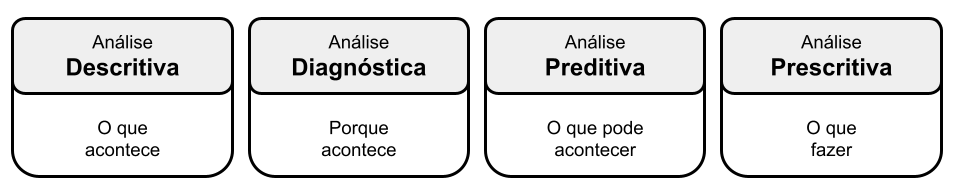
\includegraphics[scale=0.4]{figuras/tipos_analise_dados.png}
    \label{fig:tipos_analise_dados}
    \legend{Fonte: Adaptado de \citeonline{marquesone2016big}.}
\end{figure}


Essencialmente, as análises de dados podem ser divididas em quatro finalidades distintas: descritivas, diagnósticas, preditivas e prescritivas \cite{marquesone2016big}, ilustrada na Figura \ref{fig:tipos_analise_dados}. Foi aplicado a análise descritiva para dizer o que de fato acontece para na tentativa de entender o porque acontece, assim como a análise preditiva como previsão do que pode acorrer ou ocorre, tomando como referência dados reais coletados de forma indutiva para guiar na ação do que fazer, direcionando as etapas seguintes.

O processo de análise de dados é composto por seis etapas essenciais conforme a Figura \ref{fig:processo_analise_dados}, considerando o objeto tema de análise e algumas ferramentas (Google Forms\footnote{https://forms.google.com} e Survio\footnote{https://survio.com}) foram aplicadas para o processo de coleta, tabulação e análise.

\begin{figure}[h!]
    \caption{Processo de Análise de dados}
    \centering
    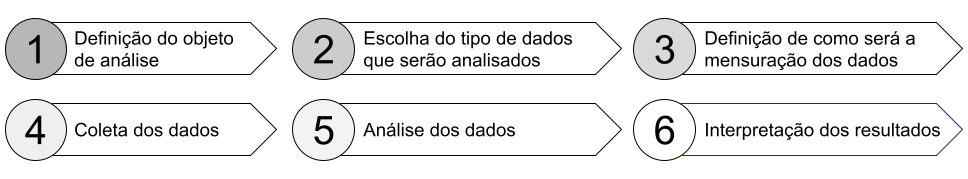
\includegraphics[scale=0.45]{figuras/processo_analise_dados.png}
    \label{fig:processo_analise_dados}
    \legend{Fonte: Adaptado de \citeonline{marquesone2016big}.}
\end{figure}

A análise utilizou para avaliar os dados encadeados nos documentos como Planos de Aula, Plano de Ensino, Plano Pedagógico de Curso (PPC) e outros documentos pertinentes como projetos interdisciplinares ou integradores e dos questionários aplicados. Por fim para \cite{marconi2017fundamentos} esta análise se divide em três etapas, compreendidas entre "interpretação, explicação e especificação", considerando cada aspecto pontual e ou categorizado.